%%%%%%%%%%%%%%%%%%%%%%%%%%%%%%%%%%%%%%%%%
% Beamer Presentation
% LaTeX Template
% Version 1.0 (10/11/12)
%
% This template has been downloaded from:
% http://www.LaTeXTemplates.com
%
% License:
% CC BY-NC-SA 3.0 (http://creativecommons.org/licenses/by-nc-sa/3.0/)
%
%%%%%%%%%%%%%%%%%%%%%%%%%%%%%%%%%%%%%%%%%

%----------------------------------------------------------------------------------------
%	PACKAGES AND THEMES
%----------------------------------------------------------------------------------------

\documentclass{beamer}

\mode<presentation> {

% The Beamer class comes with a number of default slide themes
% which change the colors and layouts of slides. Below this is a list
% of all the themes, uncomment each in turn to see what they look like.

%\usetheme{default}
%\usetheme{AnnArbor}
%\usetheme{Antibes}
%\usetheme{Bergen}
%\usetheme{Berkeley}
%\usetheme{Berlin}
%\usetheme{Boadilla}
%\usetheme{CambridgeUS}
%\usetheme{Copenhagen}
%\usetheme{Darmstadt}
%\usetheme{Dresden}
%\usetheme{Frankfurt}
%\usetheme{Goettingen}
%\usetheme{Hannover}
%\usetheme{Ilmenau}
%\usetheme{JuanLesPins}
%\usetheme{Luebeck}
\usetheme{Madrid}
%\usetheme{Malmoe}
%\usetheme{Marburg}
%\usetheme{Montpellier}
%\usetheme{PaloAlto}
%\usetheme{Pittsburgh}
%\usetheme{Rochester}
%\usetheme{Singapore}
%\usetheme{Szeged}
%\usetheme{Warsaw}

% As well as themes, the Beamer class has a number of color themes
% for any slide theme. Uncomment each of these in turn to see how it
% changes the colors of your current slide theme.

%\usecolortheme{albatross}
%\usecolortheme{beaver}
%\usecolortheme{beetle}
%\usecolortheme{crane}
%\usecolortheme{dolphin}
%\usecolortheme{dove}
%\usecolortheme{fly}
%\usecolortheme{lily}
%\usecolortheme{orchid}
%\usecolortheme{rose}
%\usecolortheme{seagull}
%\usecolortheme{seahorse}
%\usecolortheme{whale}
%\usecolortheme{wolverine}

%\setbeamertemplate{footline} % To remove the footer line in all slides uncomment this line
%\setbeamertemplate{footline}[page number] % To replace the footer line in all slides with a simple slide count uncomment this line

%\setbeamertemplate{navigation symbols}{} % To remove the navigation symbols from the bottom of all slides uncomment this line
}

\usepackage{graphicx} % Allows including images
\usepackage{booktabs} % Allows the use of \toprule, \midrule and \bottomrule in tables
\usepackage[absolute,overlay]{textpos}
\usepackage{bm}
\usepackage{breqn}

\newcommand\pro{\item[$+$]}
\newcommand\con{\item[$-$]}

%----------------------------------------------------------------------------------------
%	TITLE PAGE
%----------------------------------------------------------------------------------------

\title[Scheduling Heterogenous Multi-cores]{Scheduling Heterogenous Multi-cores} % The short title appears at the bottom of every slide, the full title is only on the title page

\author{XX} % Your name
\institute[IIT Bombay] % Your institution as it will appear on the bottom of every slide, may be shorthand to save space
{
Guide: Prof XX \\ % Your institution for the title page
\medskip
}
\date{\today} % Date, can be changed to a custom date

\begin{document}

\begin{frame}
\titlepage % Print the title page as the first slide
\end{frame}

\begin{frame}
\frametitle{Motivation}
\begin{itemize}
\item Applications with distinct requirements run on a single processor.
\item To satisfy applications' distinct requirements efficiently industry has been making heterogeneous cores.
\item Many Commercial products like ARM's big.LITTLE, NVidia's Kal-El have heterogeneous cores on a single chip.
\item Heterogeneous cores enable higher performance for a given power budget $^1$.
\item {\color{blue}{Samsung's Galaxy S}} uses ARM's big.LITTLE architecture with quad-core Cortex-A7 and quad-core Cortex-A15.
\end{itemize}
\begin{table}[!h]
\vspace{-.3cm}
\centering
\begin{tabular}[bottom]{| l | l | l |}
\hline 
Performance Efficient CPU & Cortex-A15 (OoO)\\
\hline
Power Efficient CPU  & Cortex-A7	(InO) \\
\hline
\end{tabular}
\caption{ARM's big.LITTLE: Heterogeneous Cores}
\end{table}
\tiny $^1$ S. Borkar and A. A. Chien, “The future of microprocessors,” \textit{Communications of the ACM}, vol. 54, 2011
\end{frame}


\begin{frame}
\frametitle{bzip2}
\begin{figure}
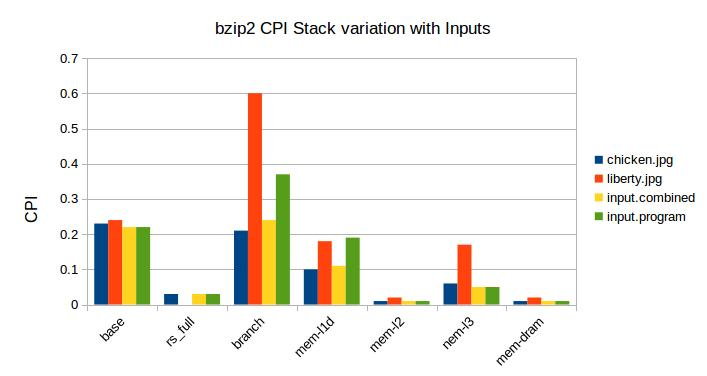
\includegraphics[width=0.98\linewidth]{bzip2}
\caption{Energy delay product for SPEC 2006 Benchmarks}
\end{figure}
\end{frame}

\begin{frame}
\frametitle{References}
\begin{itemize}
\small
\item {Kenzo Van Craeynest et al., ``Scheduling heterogeneous multi-cores through performance impact estimation (PIE)", \textit{ACM SIGARCH Computer Architecture News}, vol. 40, 2013.}
\item {R. Kumar et al., ``Single-ISA heterogeneous multi-core architectures for multithreaded workload performance", In \textit{Proceed-
ings of ISCA}, June 2004.}
\item {Stijn Eyerman et al., ``A Performance Counter Architecture for Computing Accurate CPI Components", \textit{ASPLOS}, 2006}.
\item {S. Borkar and A. A. Chien, “The future of microprocessors,” \textit{Communications of the ACM}, vol. 54, 2011}
\item Mihai et al., ``Power-Performance Modeling on Asymmetric Multi-Cores", \textit{CASES}, 2013.
\end{itemize}
\end{frame}

\begin{frame}
\Huge{\centerline{Thanks}}
\end{frame}
%----------------------------------------------------------------------------------------

\end{document} 
